
\documentclass[utf8, whale, hyperref={unicode}]{beamer}

\mode<presentation>
{
  \usetheme{Marburg}

   \setbeamertemplate{footline}
   {%
     \leavevmode%
    \hbox{\begin{beamercolorbox}[wd=.5\paperwidth,ht=2.5ex,dp=1.125ex,leftskip=.3cm 	plus1fill,rightskip=.3cm]{author in head/foot}%
    \usebeamerfont{author in head/foot}\insertshortauthor
    \end{beamercolorbox}%
    \begin{beamercolorbox}[wd=.5\paperwidth,ht=2.5ex,dp=1.125ex,leftskip=.3cm,rightskip=.3cm plus1fil]{title in head/foot}%
    \usebeamerfont{title in head/foot}\insertshorttitle \hfill p.
	\insertpagenumber\enspace i? \insertdocumentendpage\enspace
    \end{beamercolorbox}}%
  \vskip0pt%
}

  \definecolor{myBlue}{RGB}{0,170,45}
\definecolor{mygreen}{cmyk}{0.61,0.01,0.1,0.5}
\setbeamertemplate{sidebar canvas right}[vertical shading][top=palette quaternary.bg,bottom=mygreen]
\addtobeamertemplate{block begin}{\pgfsetfillopacity{0.8}}{\pgfsetfillopacity{1}}
\setbeamercolor{structure}{fg=mygreen}
\setbeamercolor*{block title example}{fg=blue!50,
bg= blue!10}
\setbeamercolor*{block body example}{fg= blue,
bg= blue!5}

  \setbeamercolor{title}{fg=black}
%
%\makeatletter
%\setbeamertemplate
%\makeatother

}
 \setbeamertemplate{navigation symbols}{}

\makeatletter
\def\maxwidth{ %
  \ifdim\Gin@nat@width>\linewidth
    \linewidth
  \else
    \Gin@nat@width
  \fi
}
\makeatother

\definecolor{fgcolor}{rgb}{0.345, 0.345, 0.345}
\newcommand{\hlnum}[1]{\textcolor[rgb]{0.686,0.059,0.569}{#1}}%
\newcommand{\hlstr}[1]{\textcolor[rgb]{0.192,0.494,0.8}{#1}}%
\newcommand{\hlcom}[1]{\textcolor[rgb]{0.678,0.584,0.686}{\textit{#1}}}%
\newcommand{\hlopt}[1]{\textcolor[rgb]{0,0,0}{#1}}%
\newcommand{\hlstd}[1]{\textcolor[rgb]{0.345,0.345,0.345}{#1}}%
\newcommand{\hlkwa}[1]{\textcolor[rgb]{0.161,0.373,0.58}{\textbf{#1}}}%
\newcommand{\hlkwb}[1]{\textcolor[rgb]{0.69,0.353,0.396}{#1}}%
\newcommand{\hlkwc}[1]{\textcolor[rgb]{0.333,0.667,0.333}{#1}}%
\newcommand{\hlkwd}[1]{\textcolor[rgb]{0.737,0.353,0.396}{\textbf{#1}}}%
\usepackage{framed}
\makeatletter
\newenvironment{kframe}{%
 \def\at@end@of@kframe{}%
 \ifinner\ifhmode%
  \def\at@end@of@kframe{\end{minipage}}%
  \begin{minipage}{\columnwidth}%
 \fi\fi%
 \def\FrameCommand##1{\hskip\@totalleftmargin \hskip-\fboxsep
 \colorbox{shadecolor}{##1}\hskip-\fboxsep
     % There is no \\@totalrightmargin, so:
     \hskip-\linewidth \hskip-\@totalleftmargin \hskip\columnwidth}%
 \MakeFramed {\advance\hsize-\width
   \@totalleftmargin\z@ \linewidth\hsize
   \@setminipage}}%
 {\par\unskip\endMakeFramed%
 \at@end@of@kframe}
\makeatother
\definecolor{shadecolor}{rgb}{.97, .97, .97}
\definecolor{messagecolor}{rgb}{0, 0, 0}
\definecolor{warningcolor}{rgb}{1, 0, 1}
\definecolor{errorcolor}{rgb}{1, 0, 0}
\newenvironment{knitrout}{}{} % an empty environment to be redefined in TeX

\usepackage{alltt}
\newtheorem{pvz}{Pavyzdys}
\IfFileExists{upquote.sty}{\usepackage{upquote}}{}

\usepackage[lithuanian, english]{babel}
\usepackage[L7x]{fontenc}
\usepackage{movie15}
\usepackage{ucs}
\usepackage{lmodern}
\usepackage{amsmath}
\usepackage{hyperref}
\usepackage{amssymb}
\usepackage{bm}
\usepackage{graphicx}
\usepackage{caption}
\usepackage{xcolor}
\usepackage{subcaption}
\usepackage{lmodern}
\usetheme{PaloAlto}
\usepackage{tikz}
\usetikzlibrary{calc}
\usepackage{verbatim}
\usepackage{alltt}
\newcommand\pro{\item[$+$]}
\newcommand\con{\item[$-$]}


% special way to reach the top of the block


\newcommand{\ab}[1]{#1_{\alpha}}
\newcommand{\wab}[2][\delta]{w_{\alpha}(#2,#1)}
\newcommand{\normab}[1]{\lVert#1\rVert_{\alpha}}
\newcommand{\eps}{\varepsilon}
\newcommand{\sprod}[1]{\langle #1 \rangle}
\DeclareMathOperator{\diam}{diam}
\theoremstyle{change}\newtheorem{teorema}{Teiginys}
\theoremstyle{change}\newtheorem{salyga}{}
\DeclareMathOperator{\seq}{seq}
\DeclareMathOperator{\Var}{Var}
\DeclareMathOperator{\tr}{tr}
\usepackage[overlay]{textpos}
\bibliographystyle{elsarticle-num}


\newtheorem{defi}{\color{white}Apibr??imas:}
\newtheorem{lyg}{\color{white}}

\newcommand{\bb}{\bm{\beta}}
\newcommand{\bx}{\mathbf{x}}
\newcommand{\indf}[1]{\mathbf{1}\left( #1 \right)}

\newenvironment{myblock}[1]{\begin{textblock*}{300pt}(#1)}{\end{textblock*}}

\newenvironment<>{varblock}[2][.9\textwidth]{%
  \setlength{\textwidth}{#1}
  \begin{actionenv}#3%
    \def\insertblocktitle{#2}%
    \par%
    \usebeamertemplate{block begin}%
    }
  {\par%
    \usebeamertemplate{block end}%
  \end{actionenv}}


\usepackage{eso-pic}
  \usepackage{tikz}
  \usepackage{xcolor}



\normalsize
\title[CNN, RNN and applications]{ {CNN, RNN and applications}}

\author[P. Daniu\v{s}is, A. Indriulionis]{P. Daniu\v{s}is, A. Indriulionis}
\medskip


\date{2018 03 08}

\begin{document}
\begin{frame}
    \titlepage
\end{frame}


\begin{frame}
	\frametitle{Presentation plan}
	\begin{itemize}
	\item Konvoliuciniai NN ir pvz.
	\item Rekurentiniai NN ir pvz.
	\item Taikymas: cross modal distillation.
	\item Taikymas: image captioning.
	\item Taikymas: object detection.		
	\end{itemize}
\end{frame}	



\begin{frame}
	\frametitle{Research criteria}
Demo filmukas \href{https://www.youtube.com/watch?time_continue=40&v=R2mC-NUAmMk}{\beamergotobutton{Link}}


	\begin{itemize}
	\item Konvoliuciniai NN ir pvz.
	\item Rekurentiniai NN ir pvz.
	\item Taikymas: cross modal distillation.
	\href{https://github.com/xiaolonw/fast-rcnn-distillation}{\beamergotobutton{Link}}
	\item Taikymas: image captioning.
	\href{https://iq.intel.com/augmented-reality-can-help-blind-see/}{\beamergotobutton{Link}}
	\item Taikymas: object detection.
	\href{https://www.veritone.com/insights/object-recognition-technology-help-blind-people-navigate/}		{\beamergotobutton{Link}}
	\end{itemize}
\end{frame}	


\begin{frame}
	\frametitle{What criteria should be met for SMART prototype?}

	\begin{itemize}
	\item Type of usage: Indoor/Outdoor recognition
	\item Type of sensors
	\item Accuracy
	\item Costs
	\item Prototype limitations
	\item Working regime: Day/Night
	\item Object detection range: Min/Max
	\item Objects Classification:  Static/Dynamic
	\item Used Techniques: for Classification, Recognition, Detection, Localization
	\item Object Detection: Real time/Static	
	\end{itemize}

\end{frame}

%
\begin{frame}
\frametitle{Image Preprocessing to Sentence}
  \hfil\hfil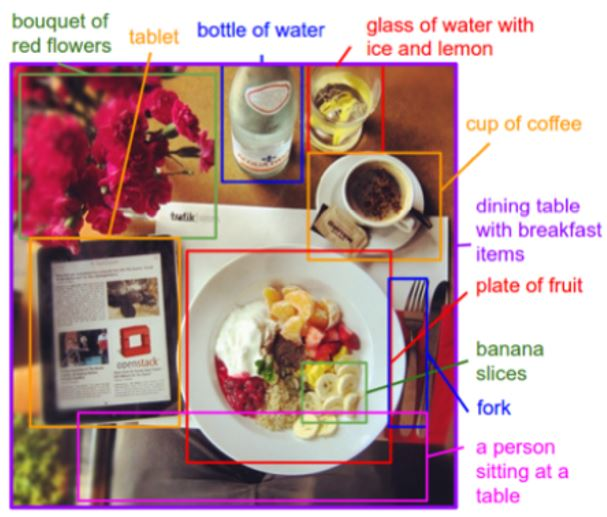
\includegraphics[width=5cm]{image/Image2Text.jpg}\newline
  \null\hfil\hfil\makebox[5cm]{Preprocessing image to text}\newline
  \vfil
  \hfil\hfil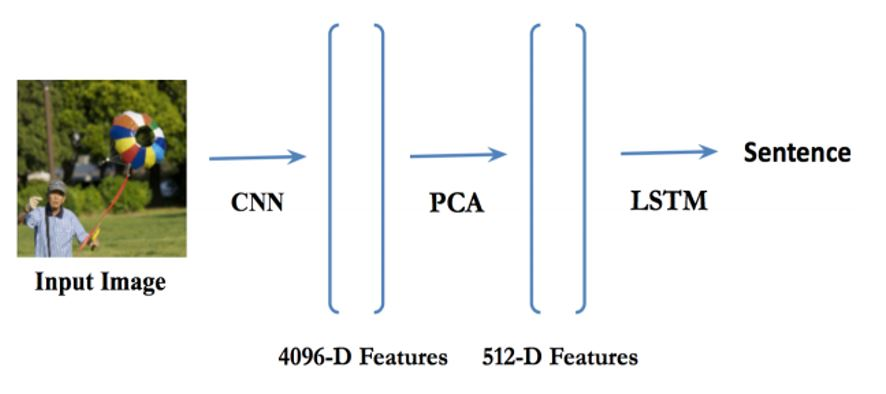
\includegraphics[width=3cm]{image/Image2Sentence_Schema.jpg}\hfil\hfil
    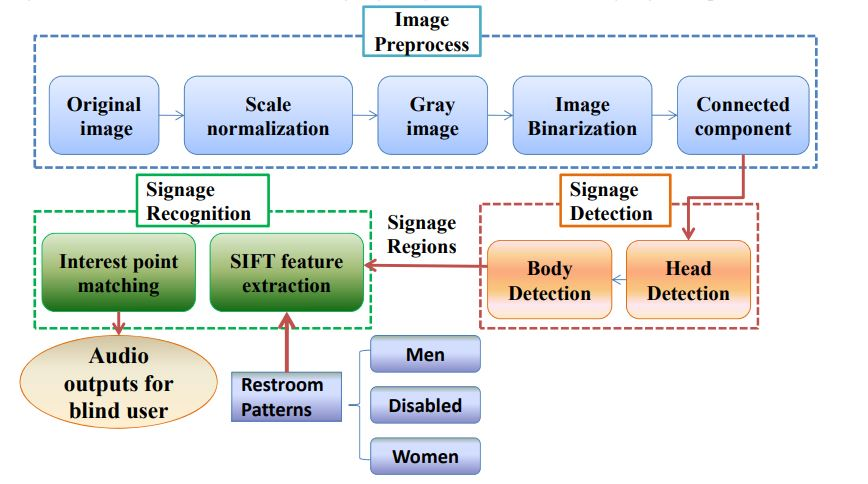
\includegraphics[width=3cm]{image/ImageProcessing.jpg}\newline
  \null\hfil\hfil\makebox[5cm]{Image preprocessing logical schema}
    \hfil\hfil\makebox[5cm]{Image preprocessing algorithm schema}
\end{frame}



\begin{frame}
\frametitle{CNN Framework and applications}
    \begin{figure}[ht]
        \begin{minipage}[b]{0.45\linewidth}
            \centering
            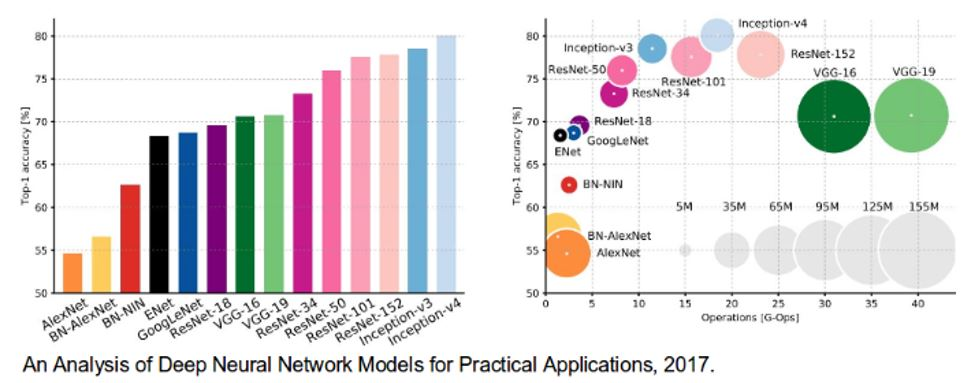
\includegraphics[width=\textwidth]{image/PracticalApplications.jpg}
            \caption{Deep Neural Networks for practical applications}
            \label{fig:PracApp}
        \end{minipage}
        \hspace{0.5cm}
        \begin{minipage}[b]{0.45\linewidth}
            \centering
            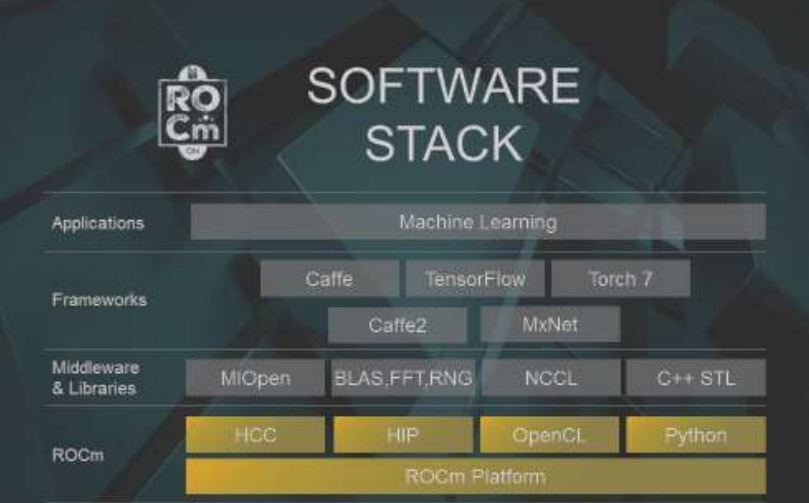
\includegraphics[width=\textwidth]{image/CNNFramework.jpg}
            \caption{Deep Neural Network Framework}
            \label{fig:DNNF}
        \end{minipage}
    \end{figure}
\end{frame}


\begin{frame}
	\frametitle{Hardware Implementation: CPU, GPU, FPGA aspects}


\end{frame}
%
%
%%GoogLENet
%%https://leonardoaraujosantos.gitbooks.io/artificial-inteligence/content/googlenet.html
%%Github: https://gist.github.com/joelouismarino/a2ede9ab3928f999575423b9887abd14
%
\begin{frame}
\frametitle{ Deep Learning Frameworks: \href{https://developer.nvidia.com/deep-learning-frameworks}{\beamergotobutton{Link}}}

	\begin{itemize}
		\item NVCaffe \href{https://github.com/BVLC/caffe}{\beamergotobutton{Link}}
		\item Caffe2
		\item  Microsoft Cognitive Toolkit (CNTK)
		\item Digits
		\item MXNet
		\item PyTorch	
		\item TensorFlow
		\item Theano
		\item Torch
		\item Keras
	\end{itemize}
\end{frame}

%
%
%
%%http://kelvinxu.github.io/projects/capgen.html
%
%
\begin{frame}
\frametitle{Image to Text to  Speech}


	\begin{itemize}
		\item CNN-based Image Feature Extractor
		\item LSTM-based Sentence Generator (LSTM learning algorithm using Simultaneous
Perturbation Stochastic Approximation (SPSA))
		\item RNN-based Sentence Generator
	\end{itemize}
\end{frame}



\begin{frame}
\frametitle{Evaluation metrics}
	\begin{itemize}
		\item BLEU (Bilingual Evaluation Understudy)
		\item METEOR (Metric for Evaluation of Translation with Explicit Ordering)
		\item CIDEr (Consensus-based Image Description Evaluation)
\end{itemize}

\end{frame}

\begin{frame}
	\frametitle{Image, Video and Audio data sets}


  \begin{itemize}
  	\item COCO \href{https://github.com/nightrome/cocostuff}{\beamergotobutton{Link}}
				\href{http://www.vision.caltech.edu/~mronchi/projects/Cocoa/}{\beamergotobutton{Link}}
	\item ImageNet \href{http://image-net.org/download-images}{\beamergotobutton{Link}}
	\item SUN	\href{http://vision.cs.princeton.edu/projects/2010/SUN/}{\beamergotobutton{Link}}
    \item Google Open Images(~9M images) \href{https://github.com/openimages/dataset}{\beamergotobutton{Link}}
	\item Youtube-8M (8M videos) \href{ https://research.google.com/youtube8m/}{\beamergotobutton{Link}}
	\item AudioSet(2M sound clips)  \href{https://research.google.com/audioset/index.html }{\beamergotobutton{Link}}
  \end{itemize}
\end{frame}


\end{document}
